\documentclass[11pt,a4paper]{article}
\usepackage{fullpage}
\usepackage{graphicx}
\usepackage{float}
\title{\textbf{Chaotic Dynamics - CSCI 5446} \\
Problem Set 1}
\author{Santhanakrishnan Ramani}
\begin{document}
\maketitle
\section*{Problem 3}
\paragraph{•}
The following figures are some interesting plots obtained by plotting $x_{n}$ vs $n$, $x_{n+1}$ vs $x_{n}$, $x_{n+2}$ vs $x_{n}$, for the logistic function, $$x_{n+1} = Rx_{n}(1-x{n})$$
\begin{figure}[H]
{
The Figure \ref{fig:fp} show us that for the value of R = 2.8 and initial condition $x_{0}$ = 0.2, the system converges to a stable fixed point after some initial transient, in language of dynamical systems this is commonly referred as Fixed Point Attractor.\par
\bigskip
\centering 
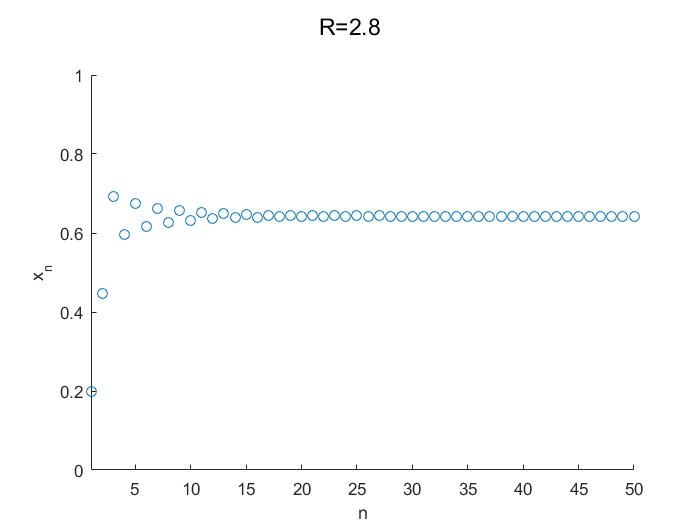
\includegraphics[scale=0.5]{images/fixed.jpg}
\caption{Fixed Point}\par\medskip
\label{fig:fp}
}
\end{figure}
\begin{figure}[H]
{
The Figure \ref{fig:2pc} show us that for the value of R = 3.2 and initial condition $x_{0}$ = 0.2, the system oscillates in two period cycle after some initial transient, the period-2 cycle is clearly evident from Figure \ref{fig:2pc1}, in language of dynamical systems this is commonly referred as Limit Cycle Attractor. \par\bigskip
\centering
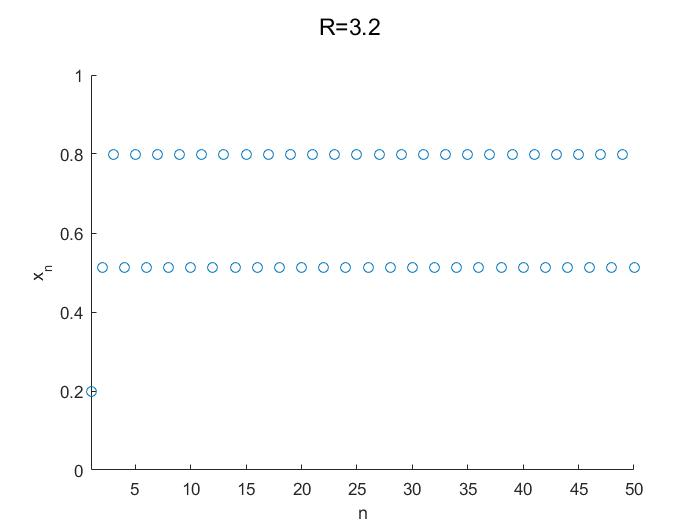
\includegraphics[scale=0.5]{images/2-period.jpg}
\caption{2-Period Cycle}\par\medskip
\label{fig:2pc}
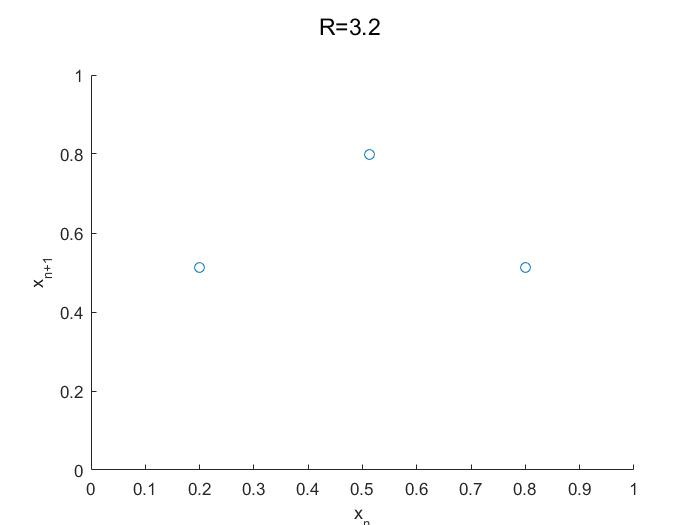
\includegraphics[scale=0.5]{images/2-period1.jpg}
\caption{2-Period Cycle}\par\medskip
\label{fig:2pc1}
}
\end{figure}
\begin{figure}[H]
{
The Figure \ref{fig:cb} and \ref{fig:cb1} show us that for the value of R = 3.97 the system exhibits Chaotic Behavior, and the behavior is highly dependent on the initial condition which is evident from the below two figures. \par\bigskip
\centering
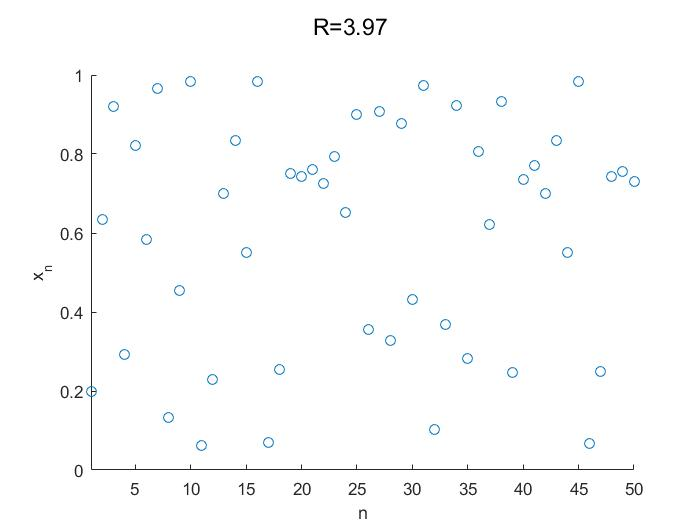
\includegraphics[scale=0.5]{images/chaotic.jpg}
\caption{Chaotic Behavior $x_{0}=0.2$}\par\medskip
\label{fig:cb}
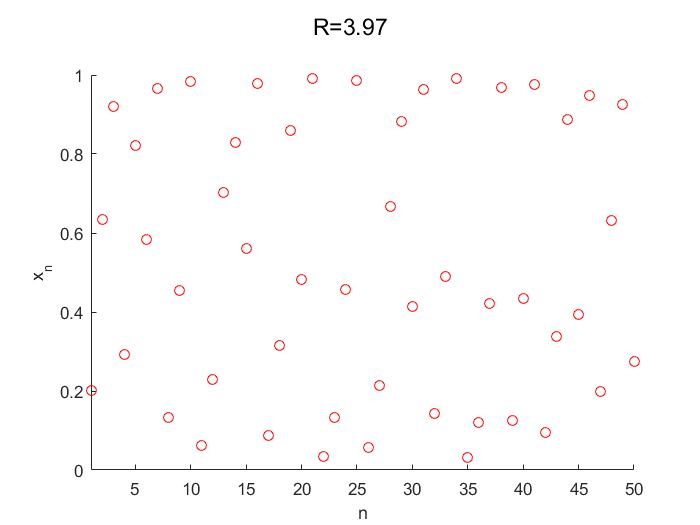
\includegraphics[scale=0.5]{images/chaotic1.jpg}
\caption{Chaotic Behavior $x_{0}=0.200001$}\par\medskip
\label{fig:cb1}
}
\end{figure}
\begin{figure}[H]
The Figure \ref{fig:r4} show us the system behavior for the value of R = 4 and $x_{0} = 0.2$, it is clearly evident from the $x_{n}$ vs $n$ graph the behavior is chaotic. The $x_{n+1}$ vs $x_{n}$ and $x_{n+2}$ vs $x_{n}$ plots shows the stretching and folding structure of the logistic map.  \par\bigskip
\centering
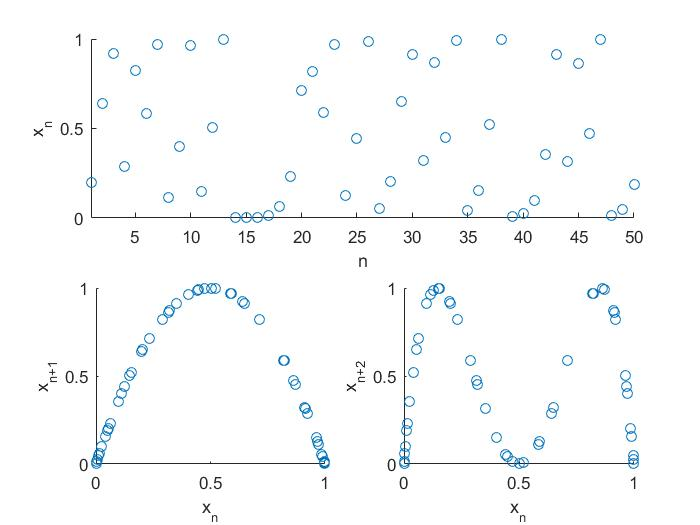
\includegraphics[scale=0.60]{images/r4.jpg}
\caption{R = 4}
\label{fig:r4}
\end{figure}
\paragraph{•}
\textbf{When R $>$ 4?}\\ 
\par\medskip
In this case, the function value goes out of the interval [0,1] and the system starts to diverge and reaches infinity for almost all initial values.
\begin{figure}[H]
\centering
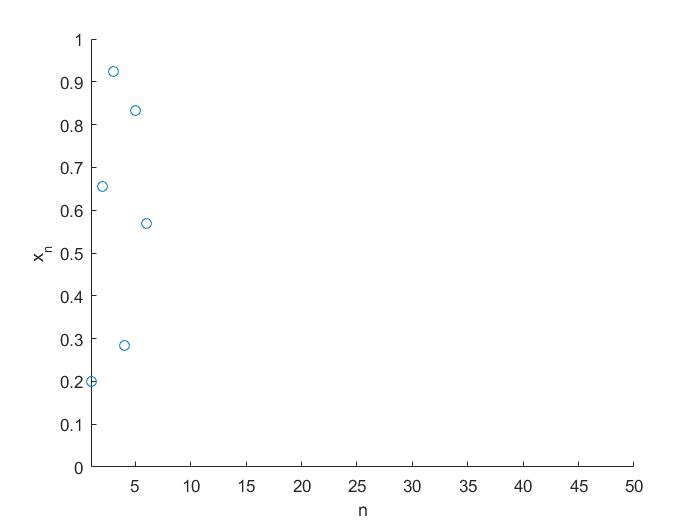
\includegraphics[scale=0.3]{images/rg4.jpg}
\caption{R $>$ 4}
\label{fig:rg4}
\end{figure}
\newpage
\paragraph{•}
\textbf{When R $=$ 2.5?}\\ 
\par\medskip
In this case the system behavior/trajectory is identical after some initial transient for any initial condition. This is evident from Figure \ref{fig:boa}, all systems with the different initial condition converges to the same stable fixed point. In Dynamical Systems terminology this is called the \textbf{basin of attraction}. 
\begin{figure}[H]
{
\centering
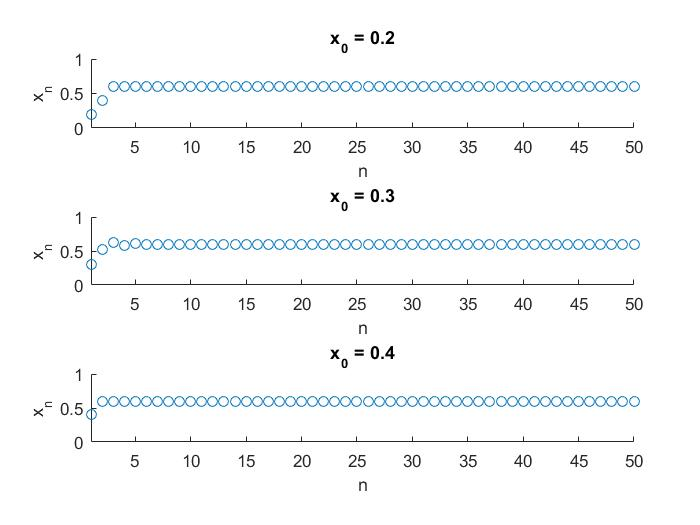
\includegraphics[scale=0.70]{images/boa.jpg}
\caption{R = 2.5}
\label{fig:boa}
}
\end{figure}
\end{document}
